During the work of this thesis around 300 movies of particles have been recorded with gradual improvements to the setup in terms of density matching, particle density, bubble elimination etc. In this section we will present the data from three movies of two different particles. One referred to as particle A, the other as particle B. The measurements in this section was done together with Alexander Laas.

\section{Particle A}

% List of parameters
%\begin{enumerate}
%
%\end{enumerate}

\begin{figure}[H]
\begin{center}
\includegraphics[width=0.7\textwidth]{figures/results/particleA/October_11_Particle_2_run_7_A.pdf}
\end{center}
\caption{Low nz almost periodic.}
\label{fig:particleA1}
\end{figure}

\begin{figure}[H]
\begin{center}
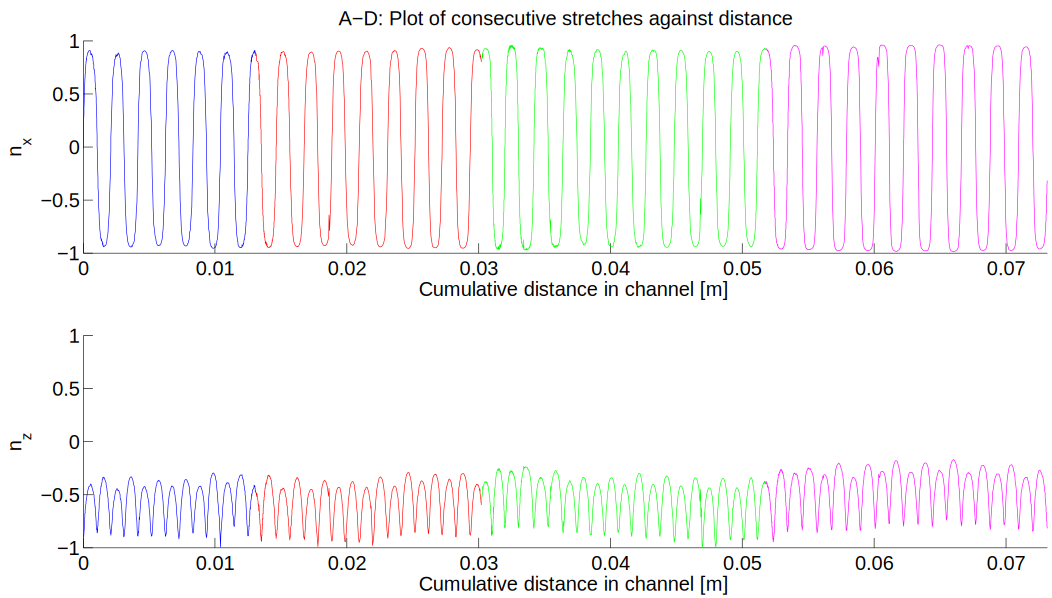
\includegraphics[width=0.7\textwidth]{figures/results/particleA/October_11_Particle_2_run_3_A.pdf}
\end{center}
\caption{High nz very periodic.}
\label{fig:particleA2}
\end{figure}

\begin{figure}[H]
\begin{center}
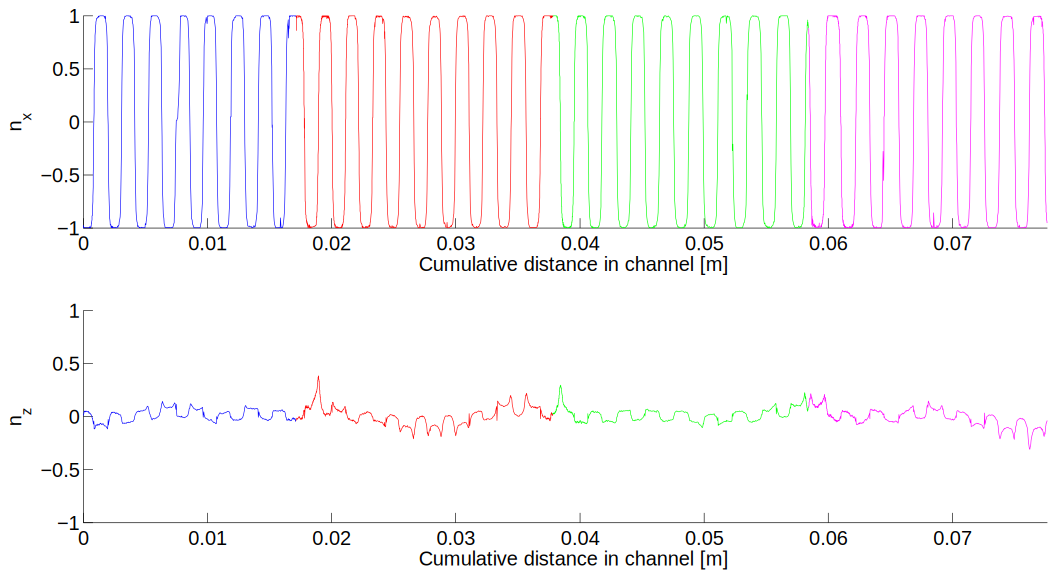
\includegraphics[width=0.7\textwidth]{figures/results/particleA/October_11_Particle_2_run_6_A.pdf}
\end{center}
\caption{Low Nz odd reversals, first peaks is bad, rest are great.}
\label{fig:particleA3}
\end{figure}

\begin{figure}[H]
\begin{center}
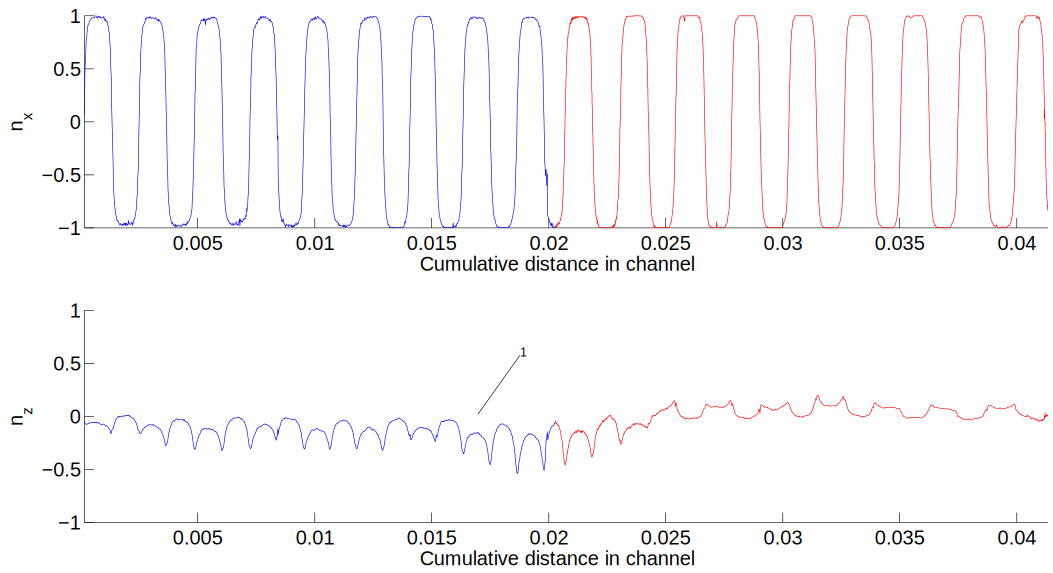
\includegraphics[width=0.7\textwidth]{figures/results/particleA/October_11_Particle_2_run_1_A.pdf}
\end{center}
\caption{Low Nz bad reversal.}
\label{fig:particleA4}
\end{figure}

\section{Particle B}

\begin{figure}[H]
\begin{center}
\includegraphics[width=0.7\textwidth]{figures/results/particleB/October_1_Particle_4_run_2_A.pdf}
\end{center}
\caption{Low nz quasiperiodic.}
\label{fig:particleB1}
\end{figure}

\begin{figure}[H]
\begin{center}
\includegraphics[width=0.7\textwidth]{figures/results/particleB/October_1_Particle_4_run_4_A.pdf}
\end{center}
\caption{High nz periodic.}
\label{fig:particleB2}
\end{figure}
